\documentclass{article}
\usepackage{cmap}
\usepackage[utf8]{inputenc}
\usepackage[english,ukrainian]{babel}
\usepackage{graphicx}
\usepackage{geometry}
\usepackage{listings}
\usepackage{float}
\usepackage{amsmath}
\usepackage{subfig}
\geometry{
	a4paper,
	left=20mm,
	right=20mm,
	top=15mm,
	bottom=15mm,
}
\lstset{
	language=c,
	tabsize=4,
	keepspaces,
	showstringspaces=false,
}
\graphicspath{ {./pictures} }
\setlength{\parindent}{4em}

\newcommand\subject{Архітектура комп'ютера}
\newcommand\lecturer{доцент кафедри ПЗ\\Крук О.Г.}
\newcommand\teacher{доцент кафедри ПЗ\\Крук О.Г.}
\newcommand\mygroup{ПЗ-22}
\newcommand\lab{2}
\newcommand\theme{Синтез та моделювання шифраторів і дешифраторів та мультиплексорів і демультиплексорів в системі Proteus}
\newcommand\purpose{Закріпити практичні навики моделювання логічних схем в середовищі системи програм Proteus; поглибити знання про основні типи комбінаційних схем: шифратори, дешифратори, мультиплексори і демультиплексори; опанувати їх синтез; дослідити роботу синтезованих схем в системі програм Proteus}

\begin{document}
\begin{normalsize}
	\begin{titlepage}
		\thispagestyle{empty}
		\begin{center}
			\textbf{МІНІСТЕРСТВО ОСВІТИ І НАУКИ УКРАЇНИ\\
				НАЦІОНАЛЬНИЙ УНІВЕРСИТЕТ "ЛЬВІВСЬКА ПОЛІТЕХНІКА"}
		\end{center}
		\begin{flushright}
			\textbf{ІКНІ}\\
			Кафедра \textbf{ПЗ}
		\end{flushright}
		\vspace{200pt}
		\begin{center}
			\textbf{ЗВІТ}\\
			\vspace{10pt}
			до лабораторної роботи № \lab\\
			\textbf{на тему}: “\textit{\theme}”\\
			\textbf{з дисципліни}: “\subject”
		\end{center}
		\vspace{112pt}
		\begin{flushright}
			
			\textbf{Лектор}:\\
			\lecturer\\
			\vspace{28pt}
			\textbf{Виконав}:\\
			
			студент групи \mygroup\\
			Коваленко Д.М.\\
			\vspace{28pt}
			\textbf{Прийняв}:\\
			
			\teacher\\
			
			\vspace{28pt}
			«\rule{1cm}{0.15mm}» \rule{1.5cm}{0.15mm} 2022 р.\\
			$\sum$ = \rule{1cm}{0.15mm}……………\\
			
		\end{flushright}
		\vspace{\fill}
		\begin{center}
			\textbf{Львів — 2022}
		\end{center}
	\end{titlepage}
		
	\begin{description}
		\item[Тема.] \theme.
		\item[Мета.] \purpose.
	\end{description}

	\section*{Індивідуальне завдання}
\begin{figure}[H]
		\centering
		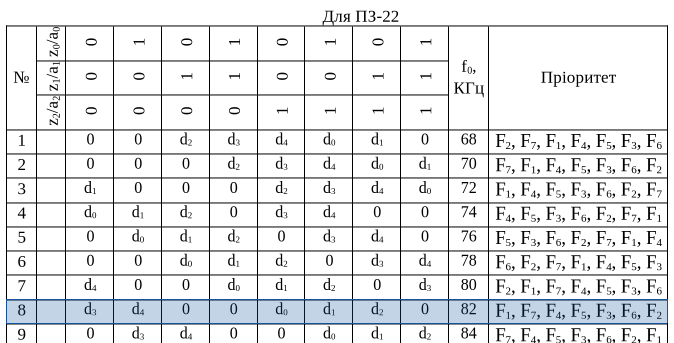
\includegraphics[scale=0.75]{v}
	\end{figure}	

	\section*{Теоретичні відомості}
	Шифратори, дешифратори, мультиплексори і демультиплексори поряд з суматорами та компараторами належать до основних типів комбінаційних цифрових схем (пристроїв). У комбінаційних пристроях (цифрових автоматах без пам’яті) вихідні сигнали в кожний момент часу повністю визначаються комбінацією поточних значень на входах і не залежать від попередніх значень вхідних сигналів.
	
	Шифратор (encoder, coder, CD) m*n - це цифровий пристрій, призначений для перетворення вхідного m-розрядного унітарного коду у вихідний n-розрядний двійковий позиційний код.
	
	Дешифратор (decoder, DC) n*m - це цифровий пристрій, призначений для перетворення вхідного n-розрядного двійкового позиційного коду у вихідний m-розрядний унітарний код.
	
	Мультиплексор (multiplexer, MUX) - це комбінаційний цифровий пристрій, призначений для комутування (перемикання) логічних сигналів від одного з n інформаційних X-входів на єдиний D-вихід.
	
	Демультиплексoр (demultiplexer, DMX) - це комбінаційний цифровий пристрій, призначений для комутування (перемикання) логічного сигналу з одного інформаційного D‑входу на один з n інформаційних Y‑виходів.
	
	\section*{Хід роботи}
	\begingroup
	\setlength{\belowdisplayskip}{-15pt}
	\setlength{\abovedisplayskip}{0pt}
	\subsection*{Період цифрового сигналу}
	\begin{large}
		\begin{gather}
			T=\frac{1}{f};\hspace{22mm}T=\frac{1}{82\text{кГц}}=\frac{1}{82000\text{Гц}}=0.0000121\text{с}\nonumber\\
			\tau=\frac{T}{8}=0.00000151\text{с}\nonumber
		\end{gather}
	\end{large}
	\subsection*{ДДНФ заданої функції}
	\begin{large}
		\begin{gather}
			F=\overline{x_2}\overline{x_1}\overline{x_0}+\overline{x_2}\overline{x_1}x_0+x_2\overline{x_1}\overline{x_0}+x_2\overline{x_1}x_0+x_2x_1\overline{x_0}	\nonumber
		\end{gather}
	\end{large}
	\endgroup

	\section*{Схема пріоритетного шифратора 8x3}	
	\begin{figure}[H]
		\centering
		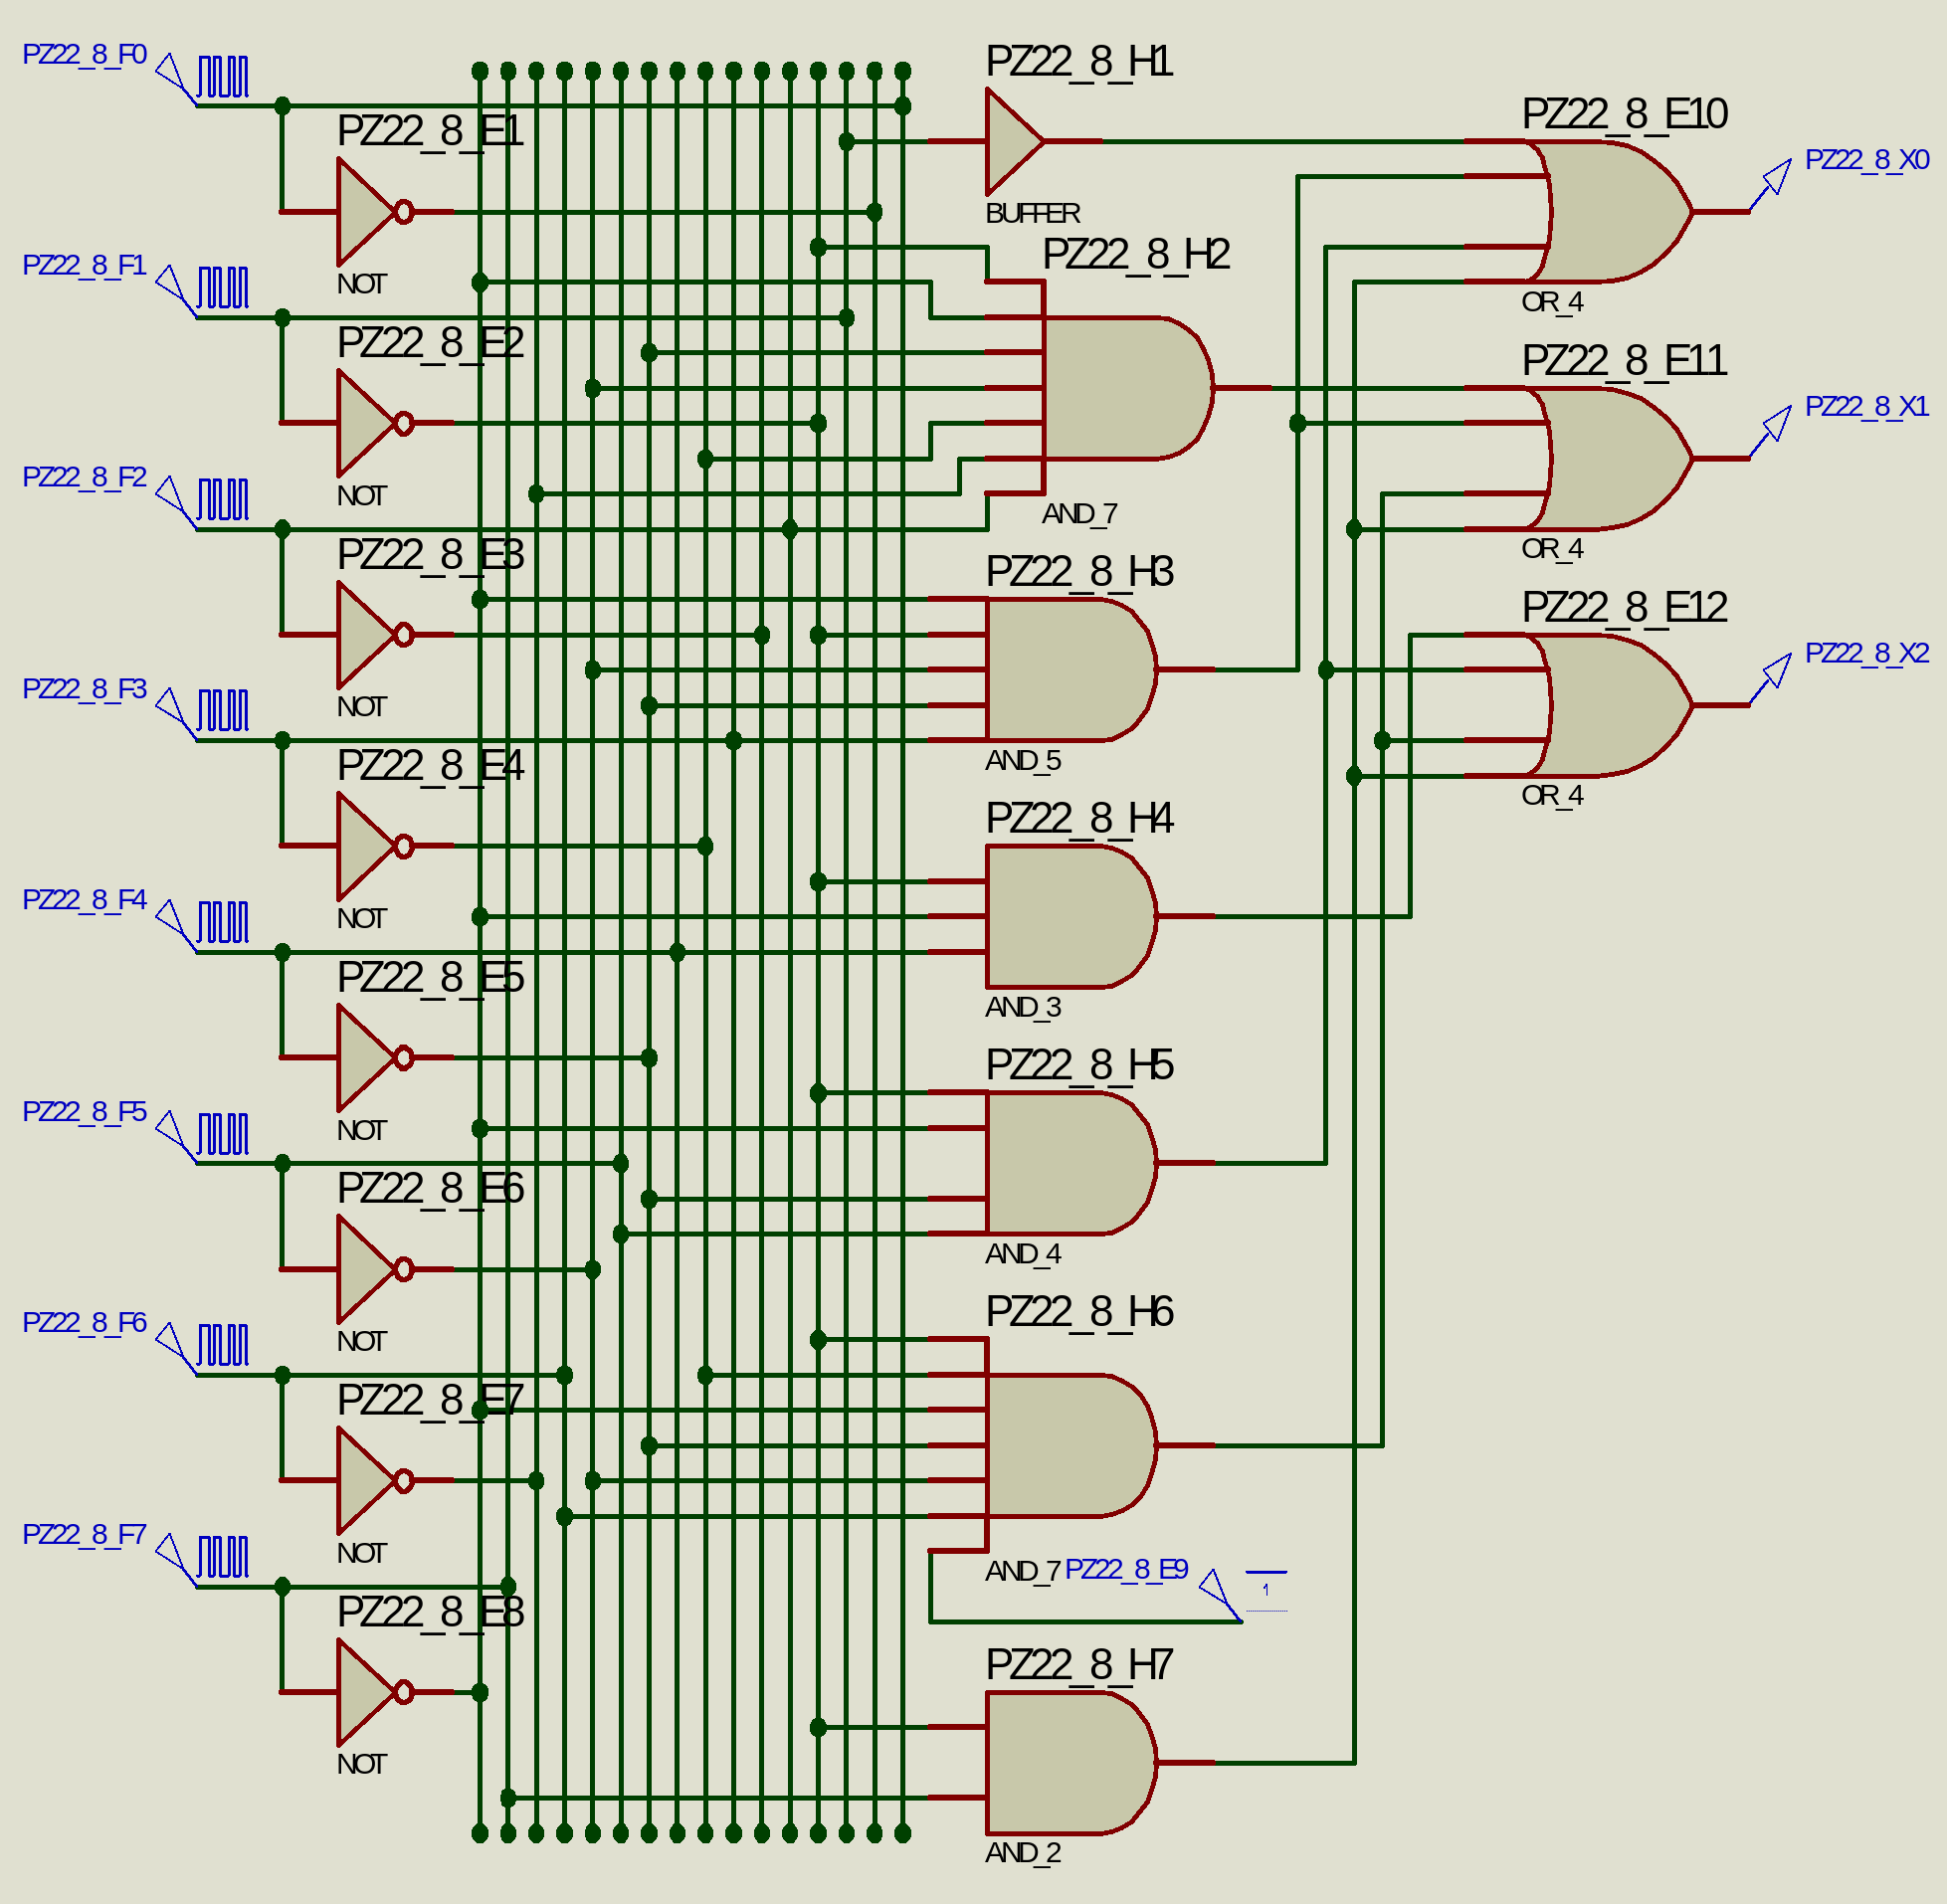
\includegraphics[scale=0.25]{s1}	
		\caption{Схема 1}
	\end{figure}

	\begin{Large}
		\begin{align}
			\begin{gathered}
				H_1 = F_1\nonumber\\		
				H_7 = \overline{F_1}\land F_7\nonumber\\
				H_4 = \overline{F_1}\land \overline{F_7}\land F_4\nonumber\\
				H_5 = \overline{F_1}\land \overline{F_7}\land \overline{F_4}\land F_5\nonumber\\
				H_3 = \overline{F_1}\land \overline{F_7}\land \overline{F_4}\land \overline{F_5}\land F_3\nonumber\\
				H_6 = \overline{F_1}\land \overline{F_7}\land \overline{F_4}\land \overline{F_5}\land \overline{F_3}\land F_6\nonumber\\
				H_2 = \overline{F_1}\land \overline{F_7}\land \overline{F_4}\land \overline{F_5}\land \overline{F_3}\land \overline{F_6}\land F_2\nonumber
			\end{gathered}
			&&
			\begin{gathered}
				X_0=F_1\lor F_3\lor F_5\lor F_7\nonumber\\
				X_0=F_2\lor F_3\lor F_6\lor F_7\nonumber\\
				X_0=F_4\lor F_5\lor F_6\lor F_7\nonumber
			\end{gathered}
		\end{align}
	\end{Large}

	\section*{Генератори до схеми приорітетного шифратора 8x3}
	\begin{figure}[H]
		\centering
		\subfloat[Генератор F0]{{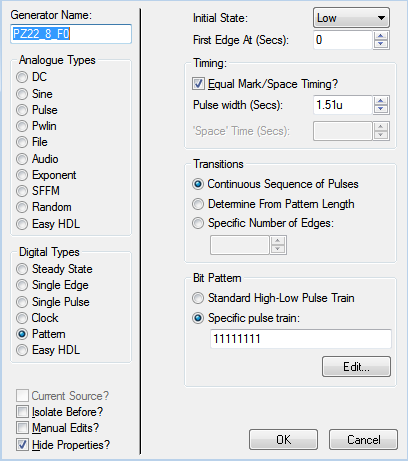
\includegraphics[width=0.45\textwidth]{f0}}}
		\hspace{5px}
		\subfloat[Генератор F1]{{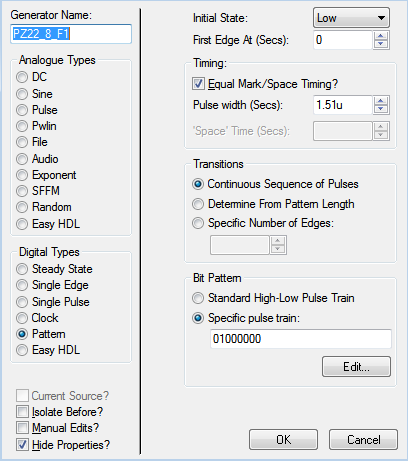
\includegraphics[width=0.45\textwidth]{f1}}}
		
		\subfloat[Генератор F2]{{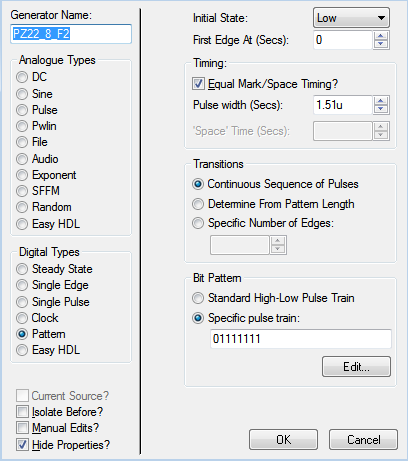
\includegraphics[width=0.45\textwidth]{f2}}}
		\hspace{5px}
		\subfloat[Генератор F3]{{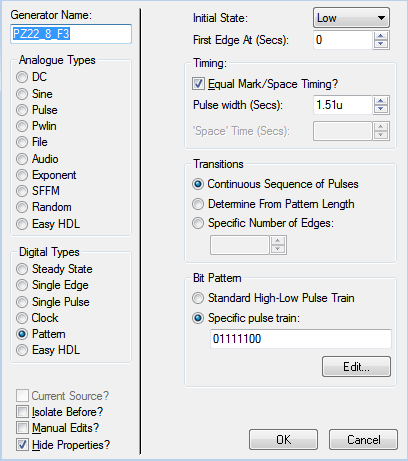
\includegraphics[width=0.45\textwidth]{f3}}}
	\end{figure}

	\begin{figure}[H]
	\centering			
		\subfloat[Генератор F4]{{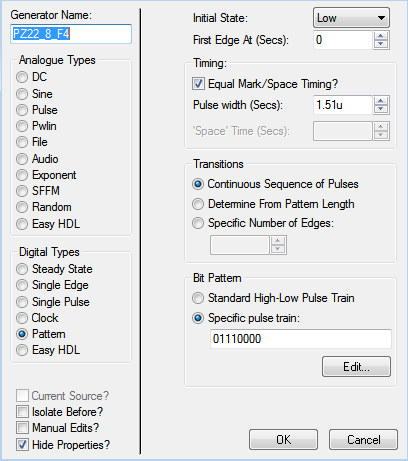
\includegraphics[width=0.45\textwidth]{f4}}}
		\hspace{5px}
		\subfloat[Генератор F5]{{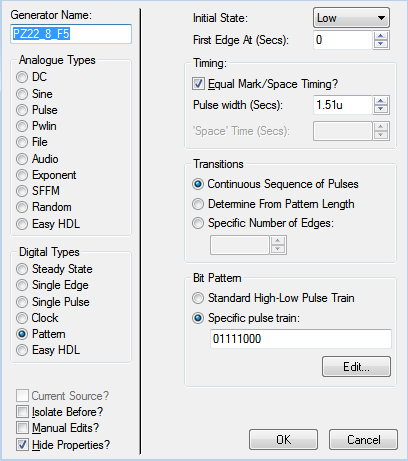
\includegraphics[width=0.45\textwidth]{f5}}}

		\subfloat[Генератор F6]{{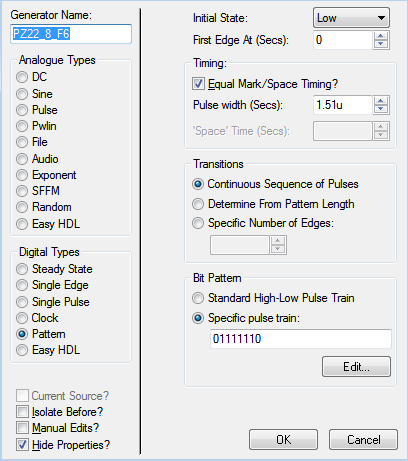
\includegraphics[width=0.45\textwidth]{f6}}}
		\hspace{5px}
		\subfloat[Генератор F7]{{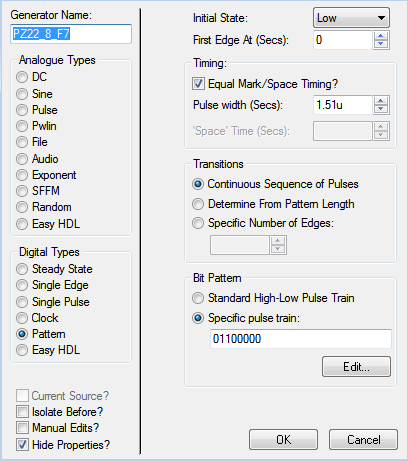
\includegraphics[width=0.45\textwidth]{f7}}}    
	\end{figure}

	\section*{Графік до схеми пріоритетного шифратора 8x3}
	\begin{figure}[H]
		\centering
		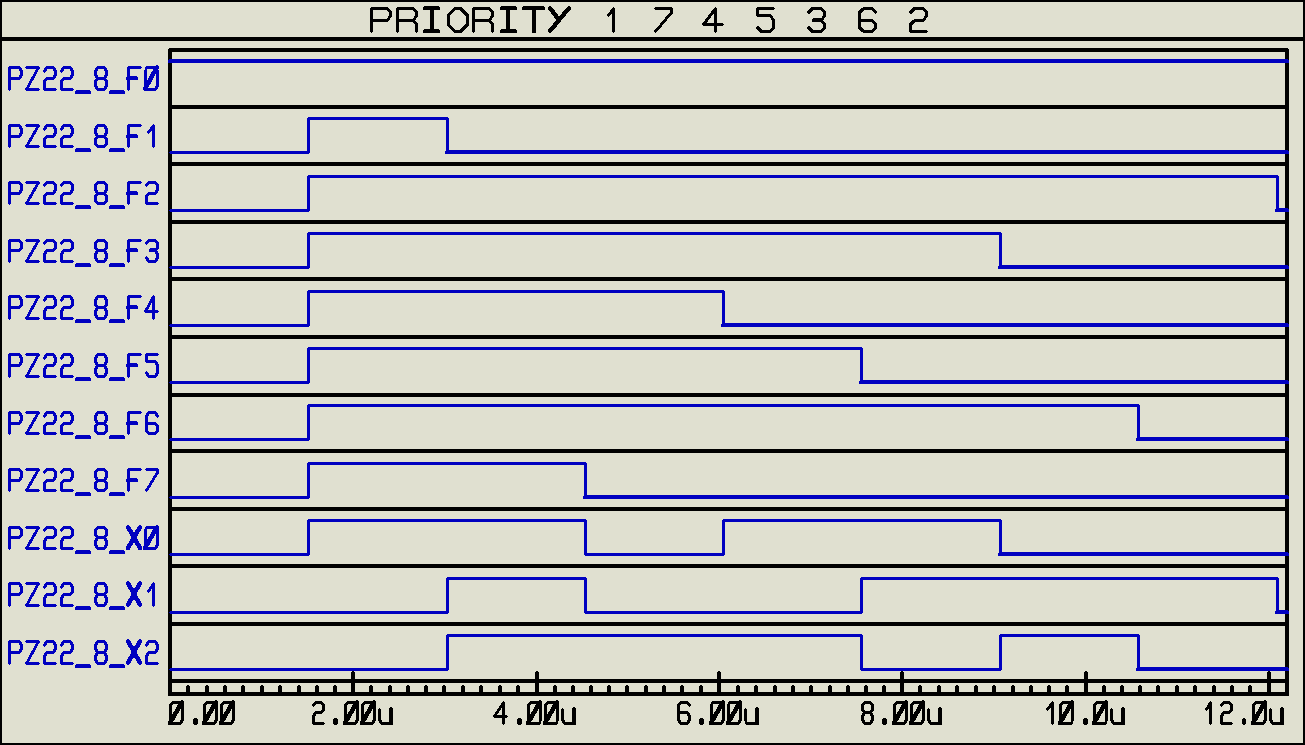
\includegraphics[scale=0.34]{g1}	
		\caption{Графік 1}
	\end{figure}

	За отриманим графіком виконання схеми пріоритетного шифратора видно, що заданий пріоритет є таким: 1, 7, 4, 5, 3, 6, 2, що повністю співпадає з заданим варіантом, отже, можна зробити виновок, що моделювання виконано правильно.

	\section*{Схема лінійного дешифратора 3x8}
	\begin{figure}[H]
		\centering
		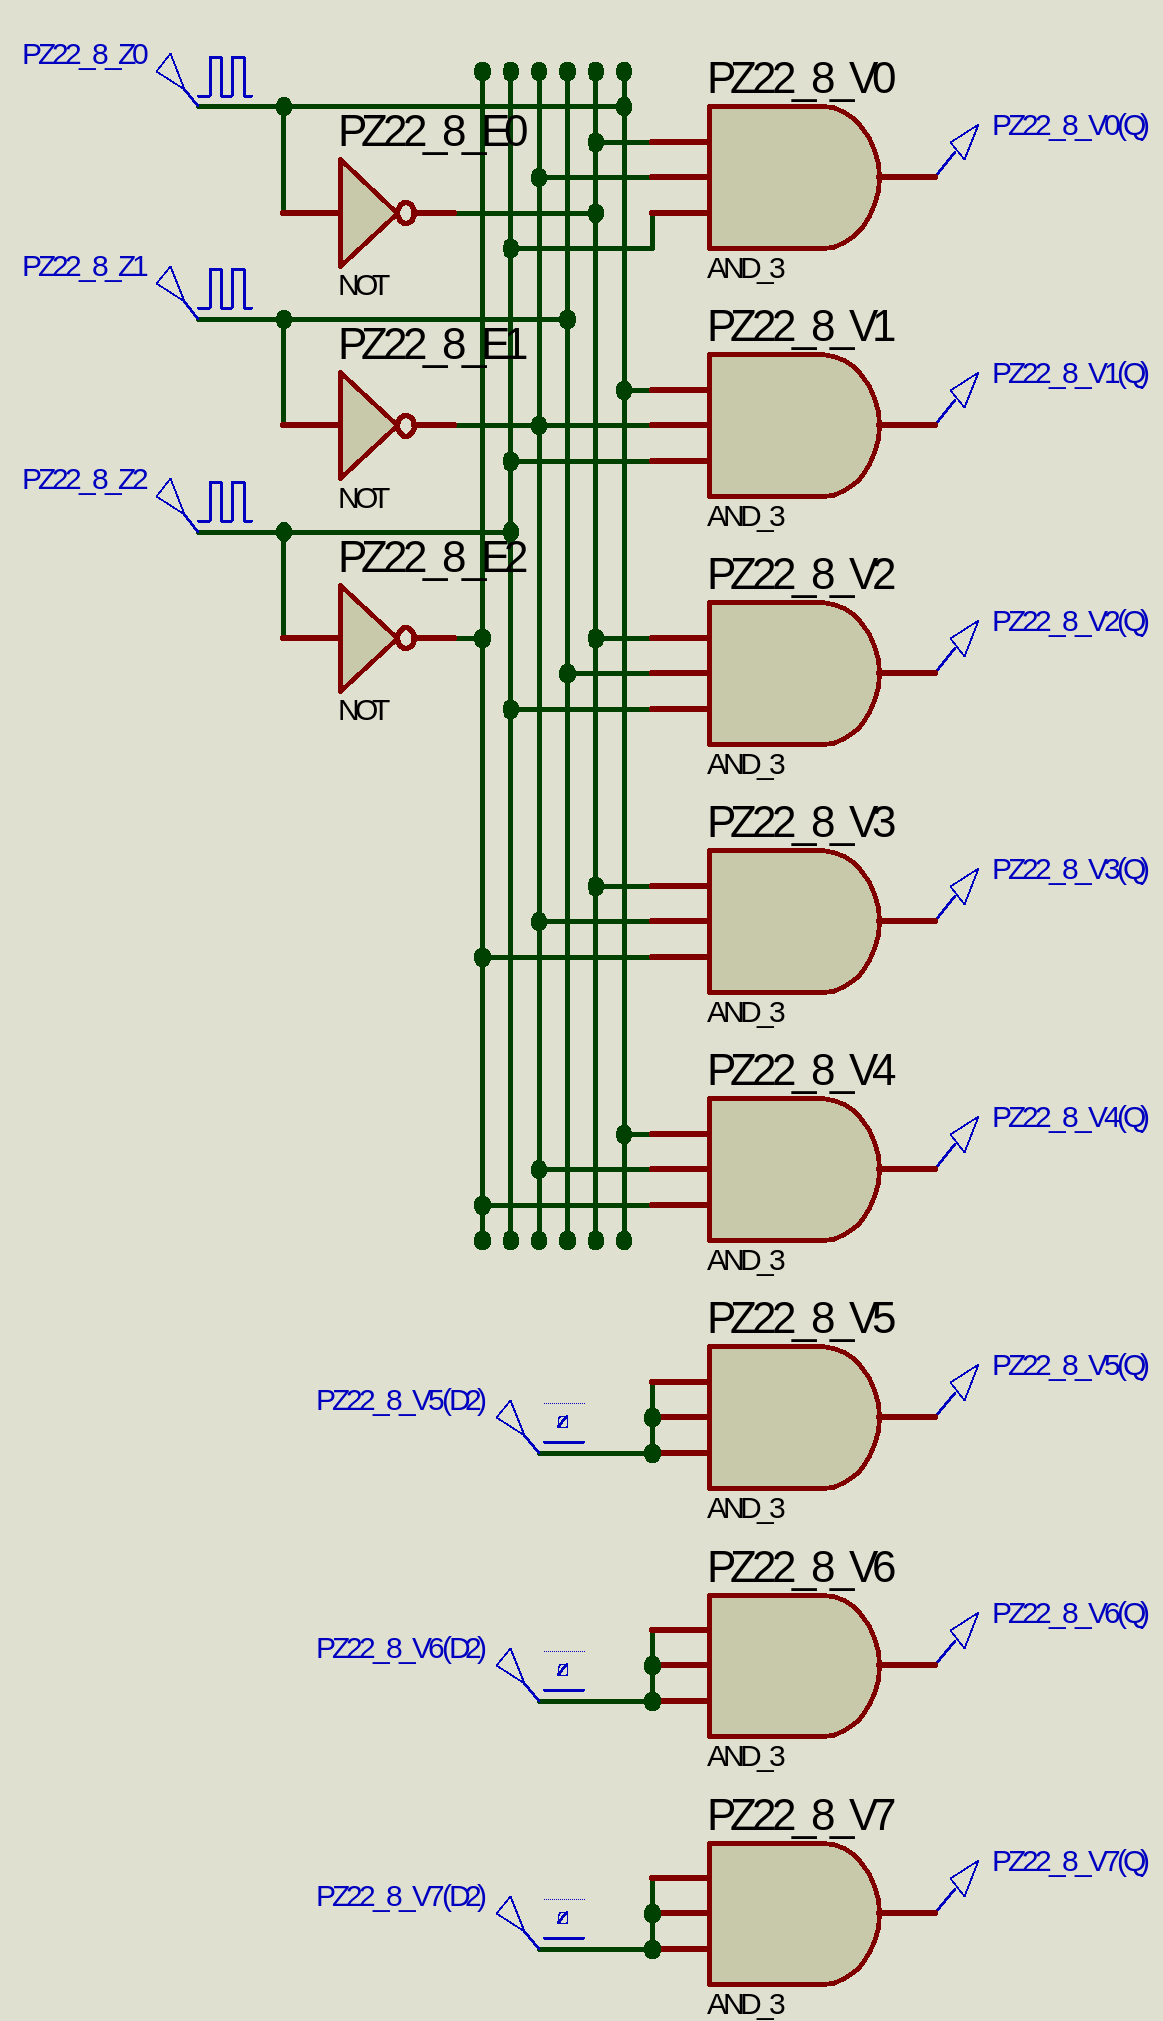
\includegraphics[scale=0.34]{s2}	
		\caption{Схема 2}
	\end{figure}

	\begin{Large}
			\begin{gather}
				V_0=Z_2\land \overline{Z_1}\land \overline{Z_0}\nonumber\\
				V_1=Z_2\land \overline{Z_1}\land Z_0\nonumber\\
				V_2=Z_2\land Z_1\land \overline{Z_0}\nonumber\\
				V_3=\overline{Z_2}\land \overline{Z_1}\land Z_0\nonumber\\
				V_4=\overline{Z_2}\land \overline{Z_1}\land Z_0\nonumber\\
				V_5=Z_2\land Z_1\land Z_0\land 0\nonumber\\
				V_6=Z_2\land Z_1\land Z_0\land 0\nonumber\\
				V_7=Z_2\land Z_1\land Z_0\land 0\nonumber
			\end{gather}
	\end{Large}

	\section*{Генератори до схеми лінійного дешифратора 3x8}
	\begin{figure}[H]
		\centering
		\subfloat[Генератор Z0]{{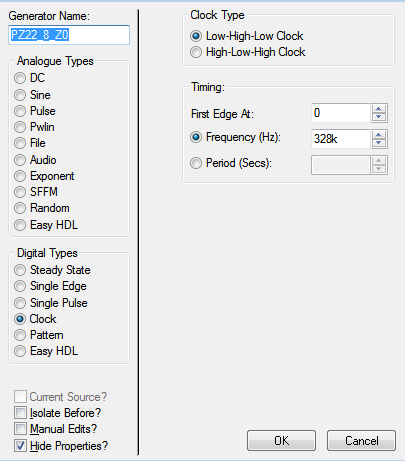
\includegraphics[width=0.43\textwidth]{z0}}}
		\hspace{5px}
		\subfloat[Генератор Z1]{{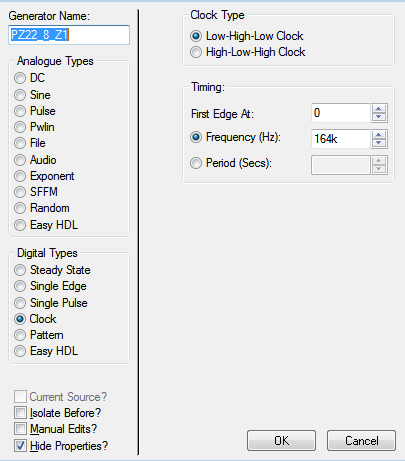
\includegraphics[width=0.43\textwidth]{z1}}}
		
		\subfloat[Генератор Z2]{{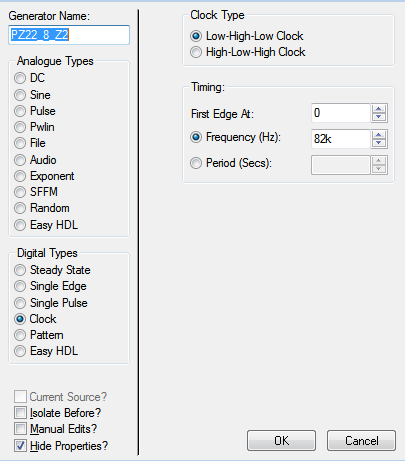
\includegraphics[width=0.43\textwidth]{z2}}}
	\end{figure}

	\section*{Графік до схеми лінійного дешифратора 3x8}
	\begin{figure}[H]
		\centering
		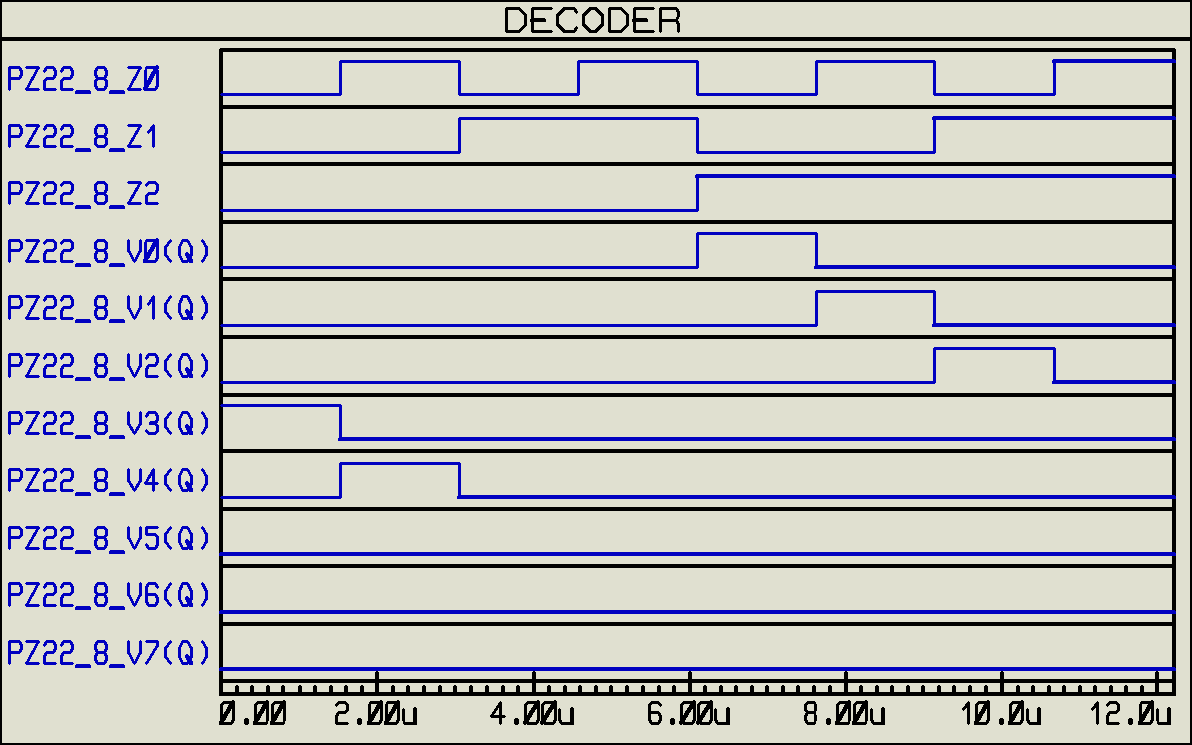
\includegraphics[scale=0.34]{g2}	
		\caption{Графік 2}
	\end{figure}

	За отриманим графіком виконання схеми лінійного дешифратора видно, що часові діаграми вхідних та вихідних сигналів на кожному з восьми проміжків відповідають заданій таблиці істиності дешифратора, отже, можна зробити виновок, що моделювання виконано правильно.

	\section*{Схема мультиплексора 5 в 1}
	\begin{figure}[H]
		\centering
		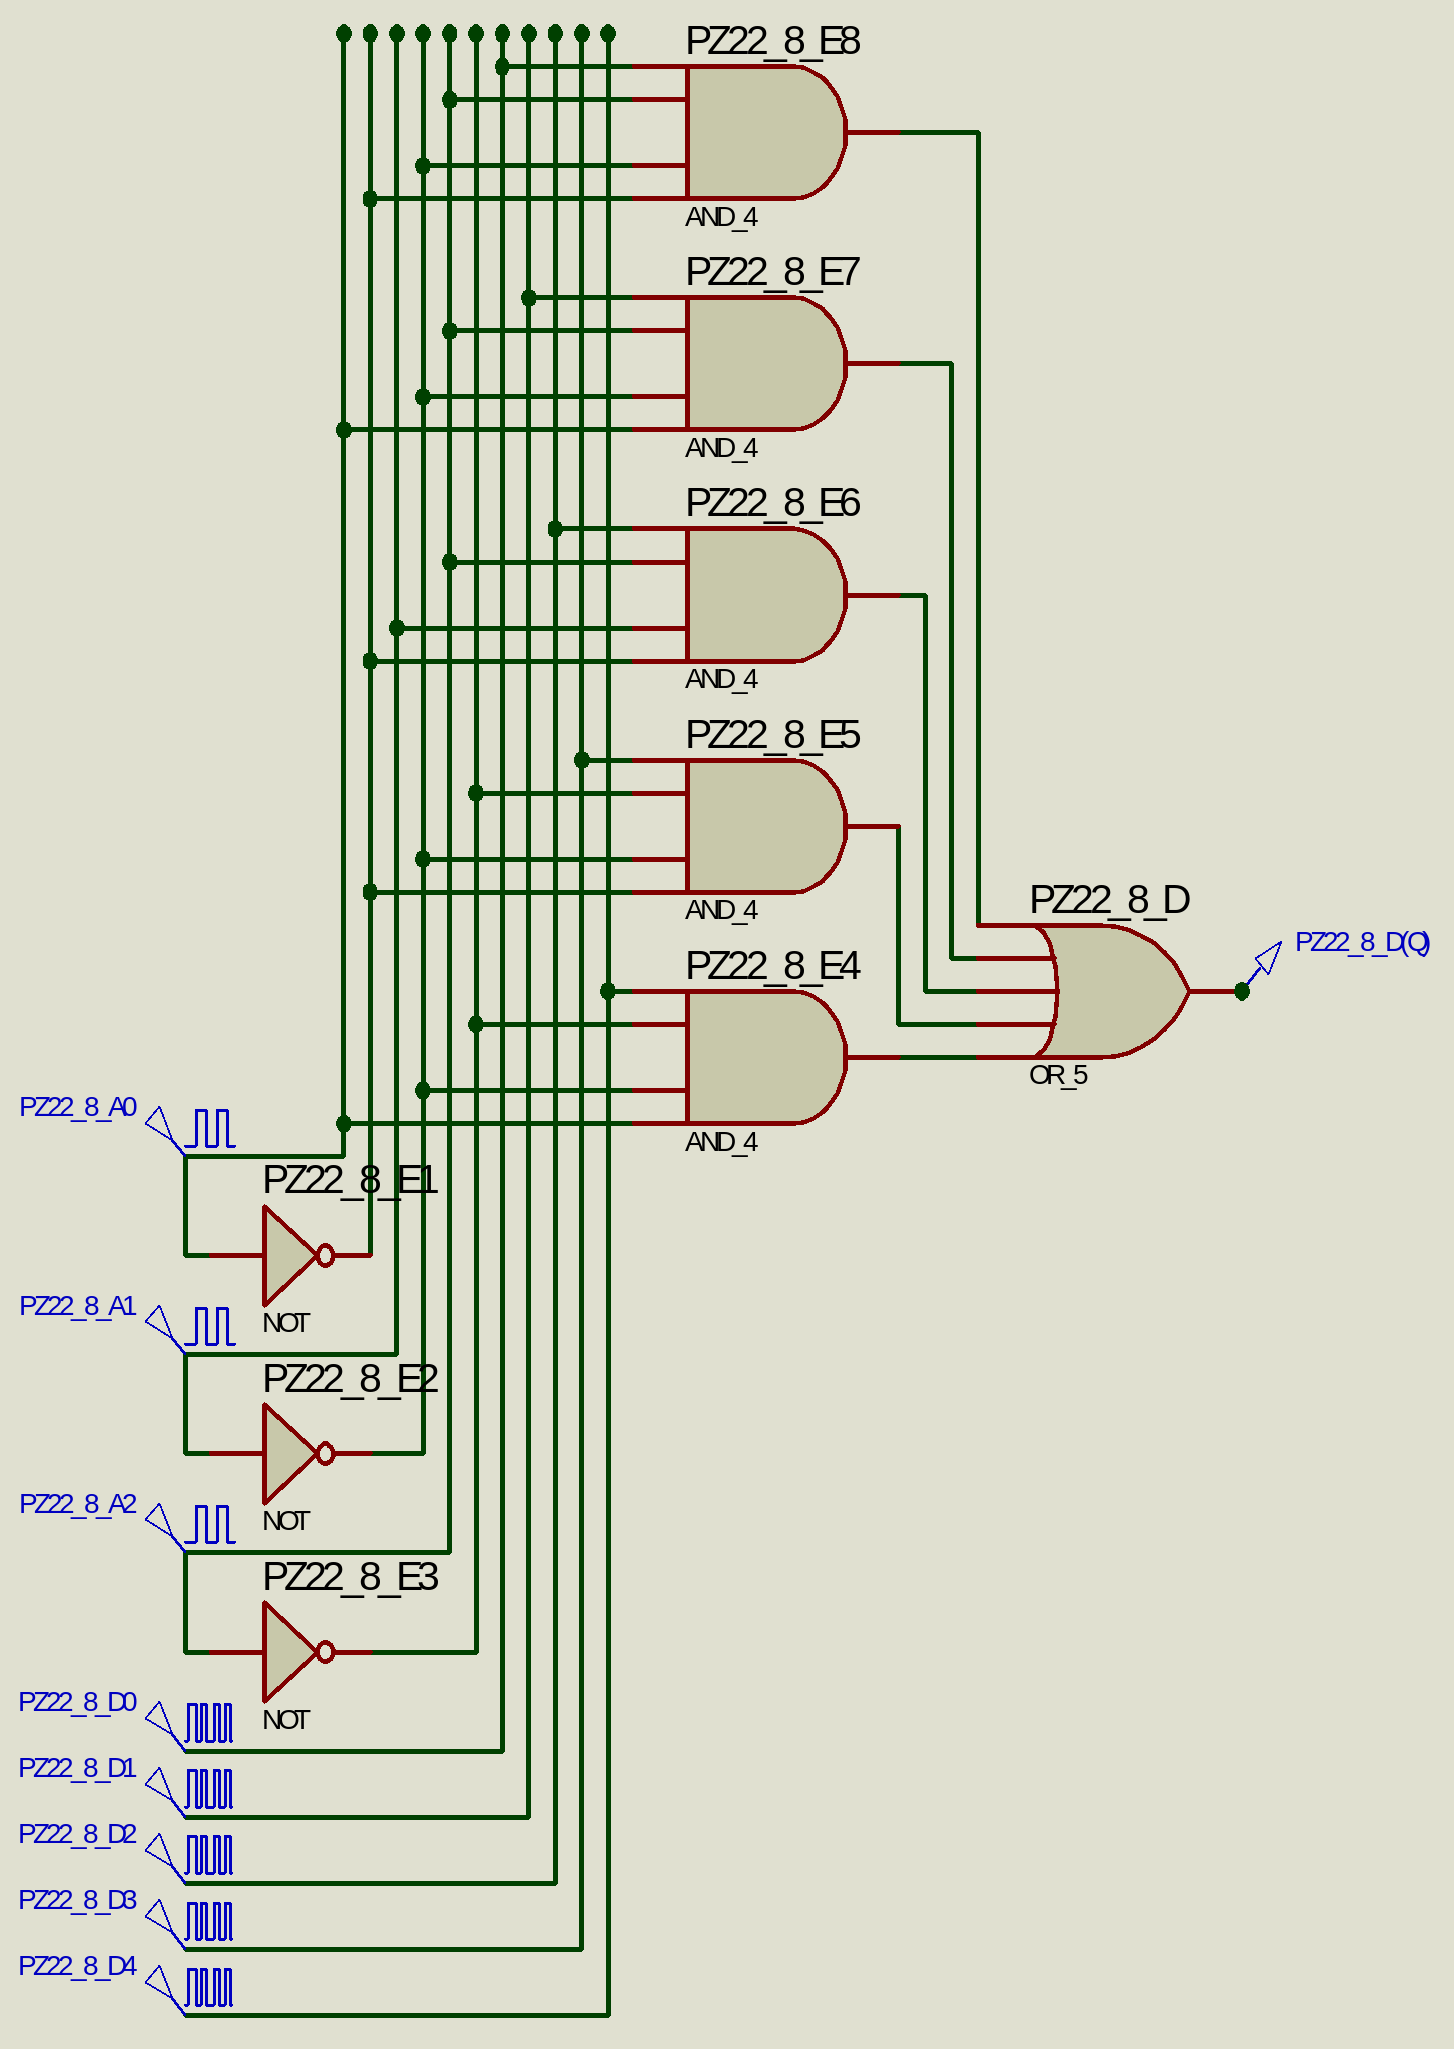
\includegraphics[scale=0.34]{s3}	
		\caption{Схема 3}
	\end{figure}

	\begin{Large}
		\begin{gather}
			D=(A_0\land\overline{A_1}\land\overline{A_2}\land D_4)\lor (\overline{A_0}\land\overline{A_1}\land\overline{A_2}\land D_3)\lor (\overline{A_0}\land A_1\land A_2\land D_2)\lor\nonumber\\\lor (A_0\land\overline{A_1}\land A_2\land D_1)\lor (\overline{A_0}\land\overline{A_1}\land A_2\land D_0)\nonumber
		\end{gather}
	\end{Large}

	\section*{Генератори до схеми мультиплексора 5 в 1}
	\begin{figure}[H]
		\centering
		\subfloat[Генератор A0]{{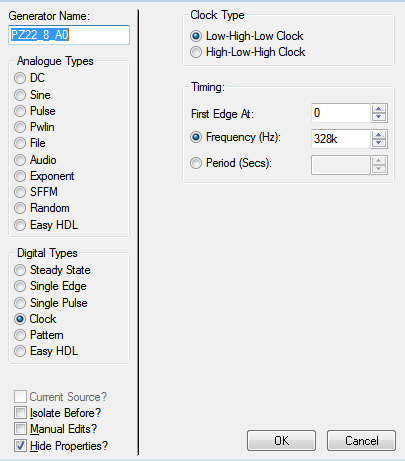
\includegraphics[width=0.45\textwidth]{a0}}}
		\hspace{5px}
		\subfloat[Генератор A1]{{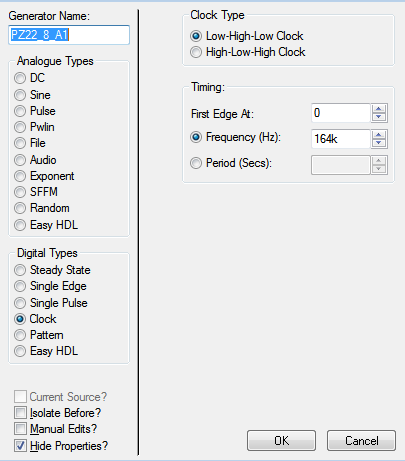
\includegraphics[width=0.45\textwidth]{a1}}}
		
		\subfloat[Генератор A2]{{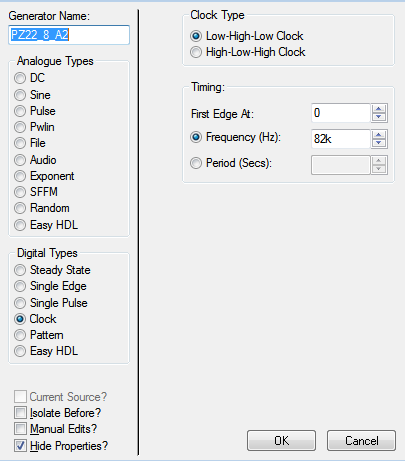
\includegraphics[width=0.45\textwidth]{a2}}}
		\hspace{5px}
		\subfloat[Генератор D0]{{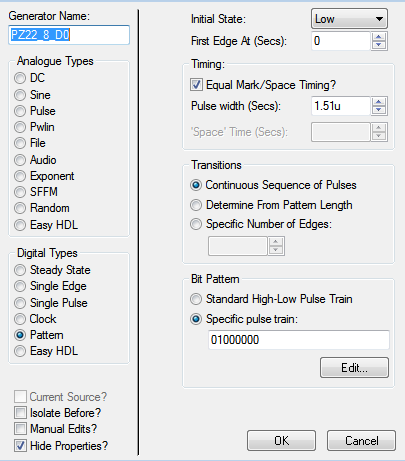
\includegraphics[width=0.45\textwidth]{d0}}}
	\end{figure}	
		
	\begin{figure}[H]
	\centering		
		\subfloat[Генератор D1]{{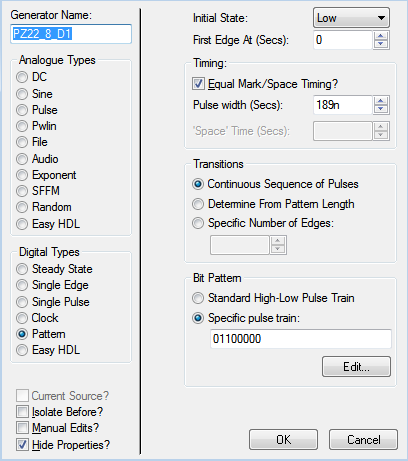
\includegraphics[width=0.45\textwidth]{d1}}}
		\hspace{5px}
		\subfloat[Генератор D2]{{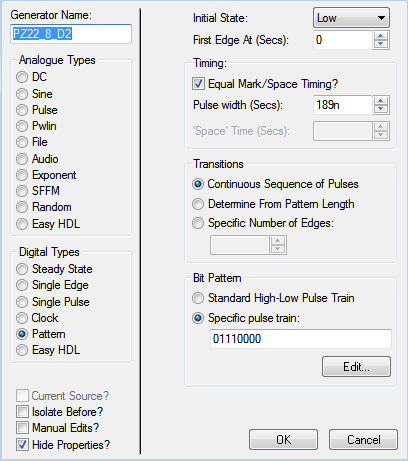
\includegraphics[width=0.45\textwidth]{d2}}}
		
		\subfloat[Генератор D3]{{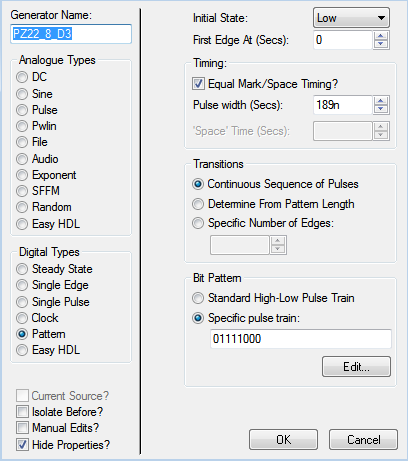
\includegraphics[width=0.45\textwidth]{d3}}}
		\hspace{5px}
		\subfloat[Генератор D4]{{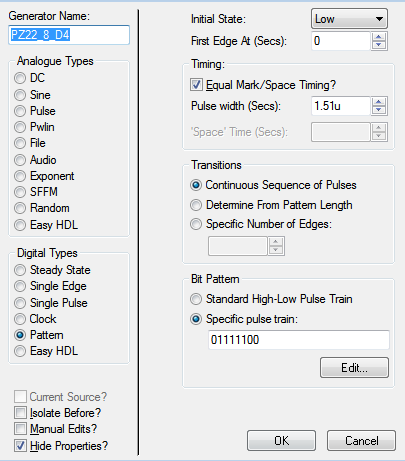
\includegraphics[width=0.45\textwidth]{d4}}}
	\end{figure}

	\section*{Графік до схеми мультиплексора 5 в 1}
	\begin{figure}[H]
		\centering
		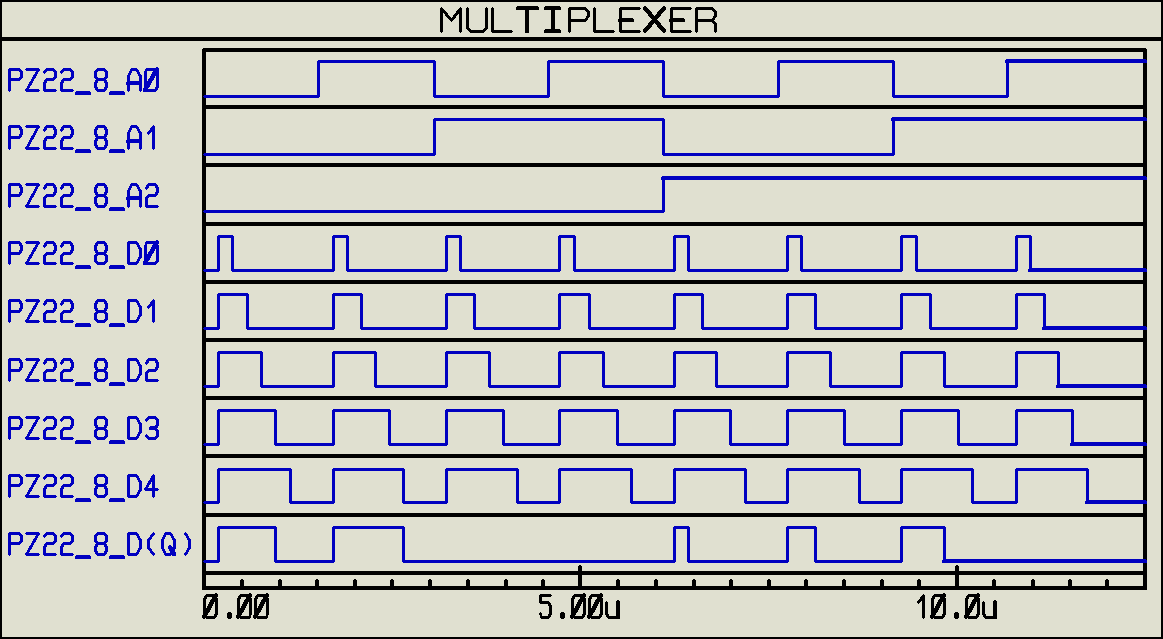
\includegraphics[scale=0.4]{g3}	
		\caption{Графік 3}
	\end{figure}

	За отриманим графіком виконання схеми мультиплексора видно, що часові діаграми вхідних та вихідних сигналів на кожному з восьми проміжків відповідають заданій таблиці істиності мультиплексора, отже, можна зробити виновок, що моделювання виконано правильно.

	\section*{Схема демультиплексора 1 в 5}
	\begin{figure}[H]
		\centering
		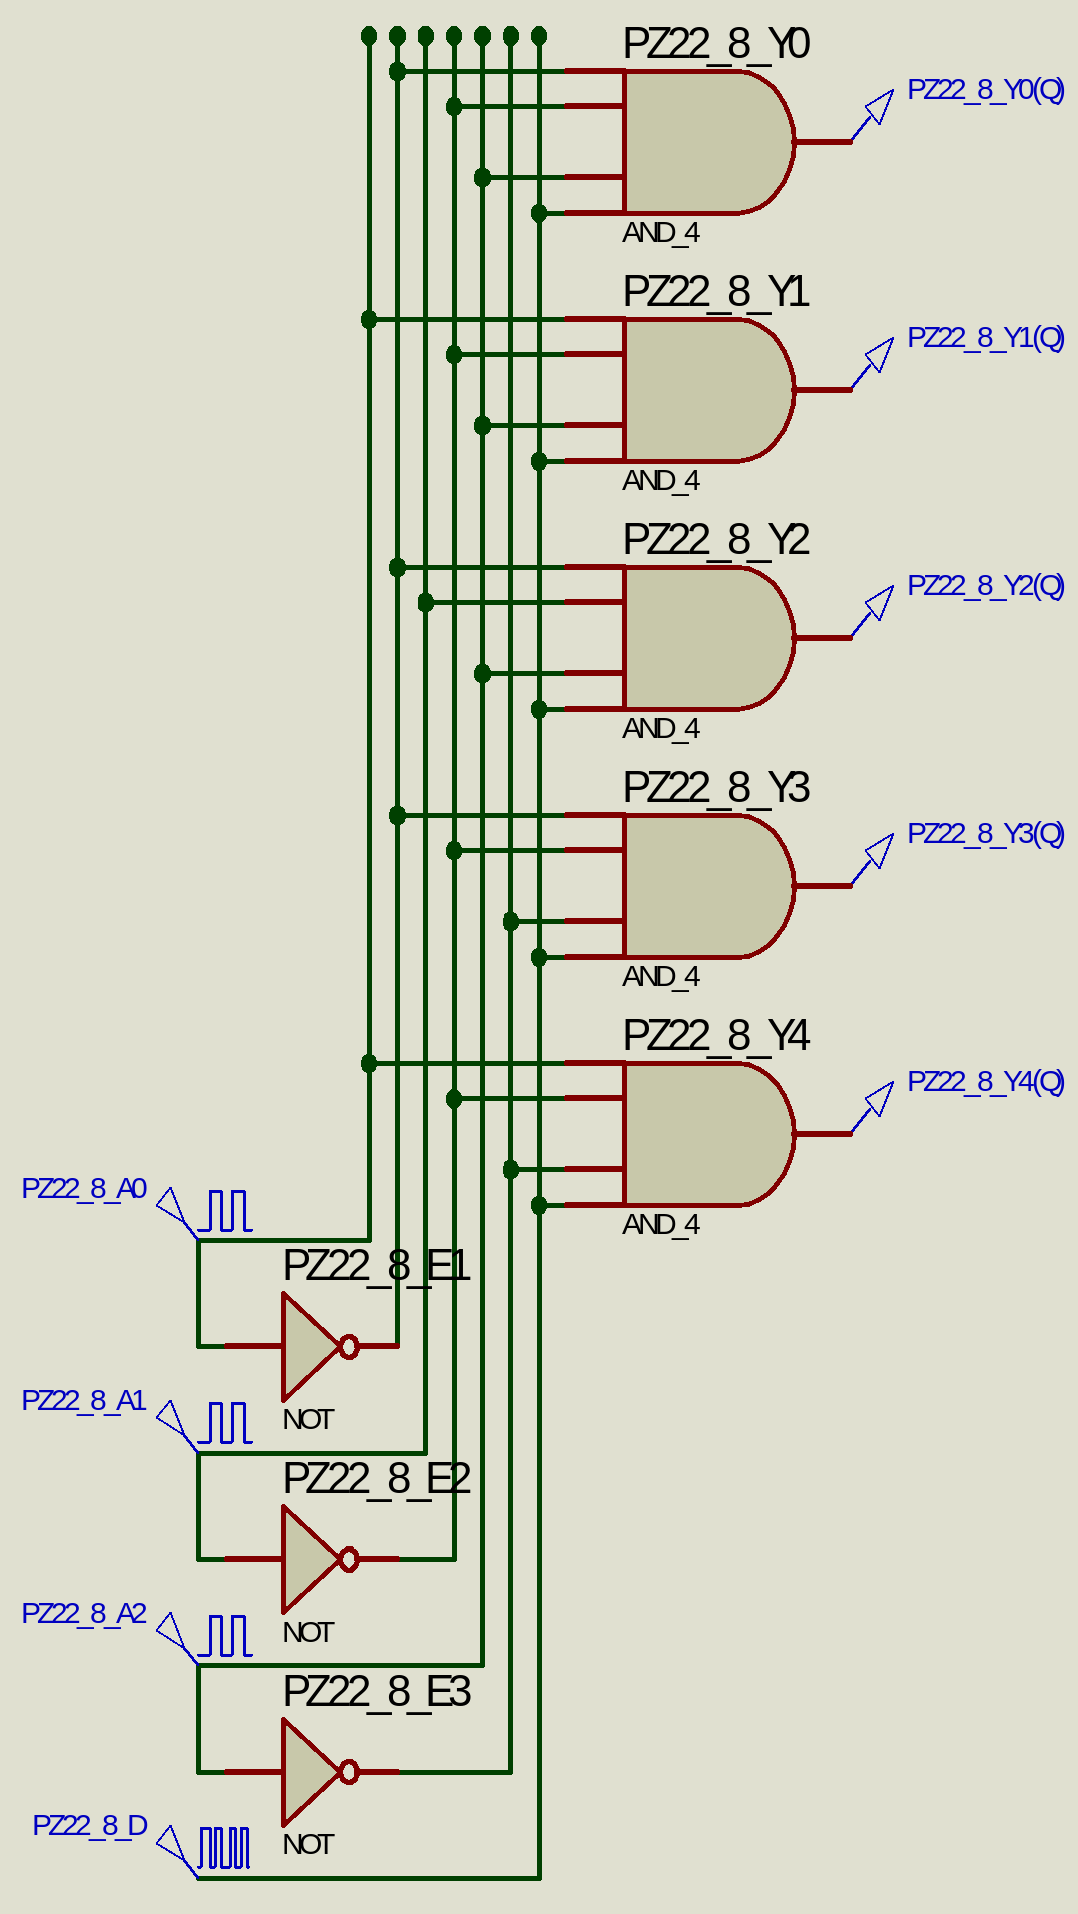
\includegraphics[scale=0.34]{s4}	
		\caption{Схема 4}
	\end{figure}

	\begin{Large}
		\begin{gather}
			Y_0=\overline{A_0}\land\overline{A_1}\land A_2\land D\nonumber\\
			Y_1=A_0\land\overline{A_1}\land A_2\land D\nonumber\\
			Y_2=\overline{A_0}\land A_1\land A_2\land D\nonumber\\
			Y_3=\overline{A_0}\land\overline{A_1}\land\overline{A_2}\land D\nonumber\\
			Y_4=A_0\land\overline{A_1}\land\overline{A_2}\land D\nonumber
		\end{gather}
	\end{Large}

	\section*{Генератори до схеми демультиплексора 1 в 5}
	\begin{figure}[H]
		\centering
		\subfloat[Генератор A0]{{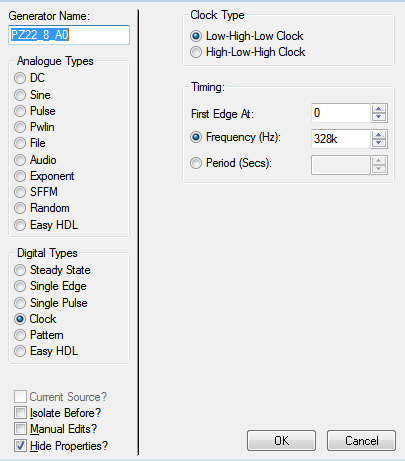
\includegraphics[width=0.45\textwidth]{a0}}}
		\hspace{5px}
		\subfloat[Генератор A1]{{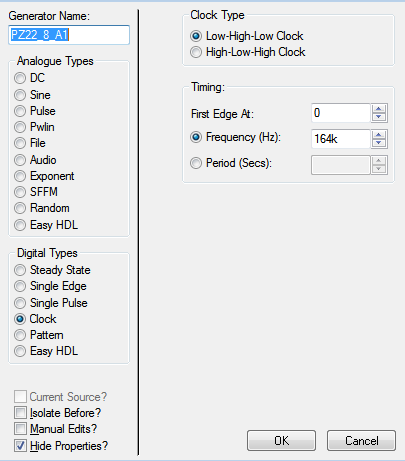
\includegraphics[width=0.45\textwidth]{a1}}}
		
		\subfloat[Генератор A2]{{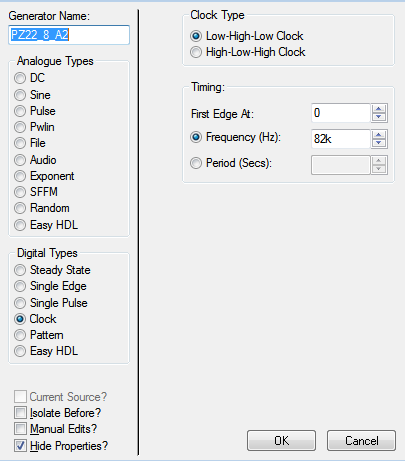
\includegraphics[width=0.45\textwidth]{a2}}}
		\hspace{5px}
		\subfloat[Генератор D]{{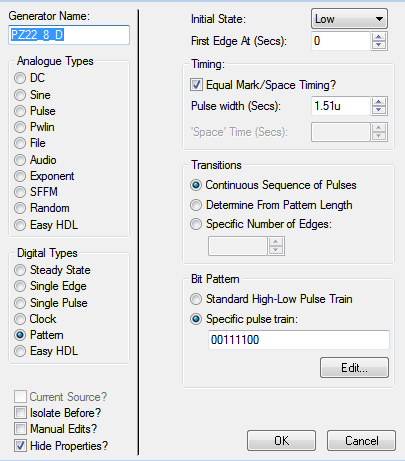
\includegraphics[width=0.45\textwidth]{d}}}
	\end{figure}	

	\section*{Графік до схеми демультиплексора 1 в 5}
	\begin{figure}[H]
		\centering
		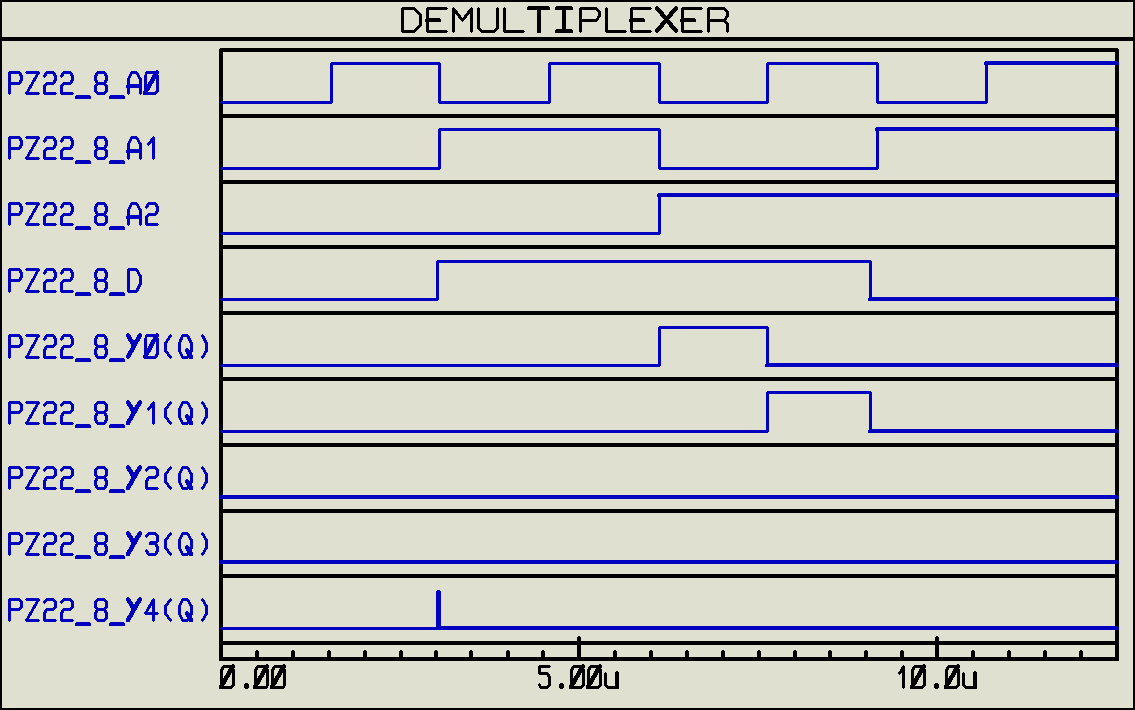
\includegraphics[scale=0.5]{g4}	
		\caption{Графік 4}
	\end{figure}

	За отриманим графіком виконання схеми демультиплексора видно, що часові діаграми вхідних та вихідних сигналів на кожному з восьми проміжків відповідають заданій таблиці істиності демультиплексора, отже, можна зробити виновок, що моделювання виконано правильно.

	\section*{Висновки}
	Під час виконання лабораторної роботи я закріпив практичні навики моделювання логічних схем в середовищі системи програм Proteus. 
	Поглибив знання про основні типи комбінаційних схем: шифратор, дешифратор, мультиплексор і демультиплексор. Опанував їх синтез. 
	
	Дослідив роботу синтезованих схем в системі програм Proteus. Змоделював графіки цих схем за заданим варіантом.
	    
\end{normalsize}
\end{document}
